\section{Graph-Metaheuristic Optimization Model for Responder Sweep Scheduling}

\vspace{-0.2cm}%在\end{table}下加一行\vspace{-1cm} 其中-1的作用是缩短与下方文字距离的 切记！必须是负数

\subsection{The Abstraction of Graph Theory}

How to assign firefighters and determine the order in which firefighters travel through room to minimize the total time consumed? We attempt to abstract the objects of this problem using \textbf{graph theory}.


We consider the object of study as a connected graph, where the rooms and exits on the map form the vertex set \( V \), and edges connect these vertices. The problem requirement can also be abstracted as: assign the vertices in the vertex set \( V \) to \( m \) firefighters, allowing them to start from safe exit vertices, traverse the assigned vertices in a certain order, and then leave from some safe exit vertices. The edge weight of the graph is the time \( T_{\text{sweep}} \) for the responder to start from one point and finish checking and clearing the next point.






Based on the graph theory "node-edge-weight" abstraction system and multi-objective optimization algorithms, the model automatically completes three core tasks:


1. Room assignment of the responders

2. Path planning of each responders

3. Fitness scoring of each combined scheme


\begin{itemize}
    \item Fitness scoring of each strategy
\end{itemize}


The evaluation metric for each combined scheme is called \textbf{fitness}.
To unify dimensions, exponential decay normalization is adopted. Let the normalized fitness value be $\hat{F}$ and the maximum total time be $T_{max} = \max(T_{\text{total}})$. The normalization formula is: \(
\hat{F} = 1 - e^{-k \cdot \max(T_{\text{total}})}\), where $k > 0$: an adjustment parameter that controls the convergence speed of fitness as $\max(T_{\text{total}})$ increases.

Given the median of the maximum total time as $\max(T_{\text{total}})$, set the fitness at this point to 0.5. Solving for $k$ gives:\(k = \ln 2/\max(T_{\text{total}})\).

\begin{figure}[htbp]
    \centering
    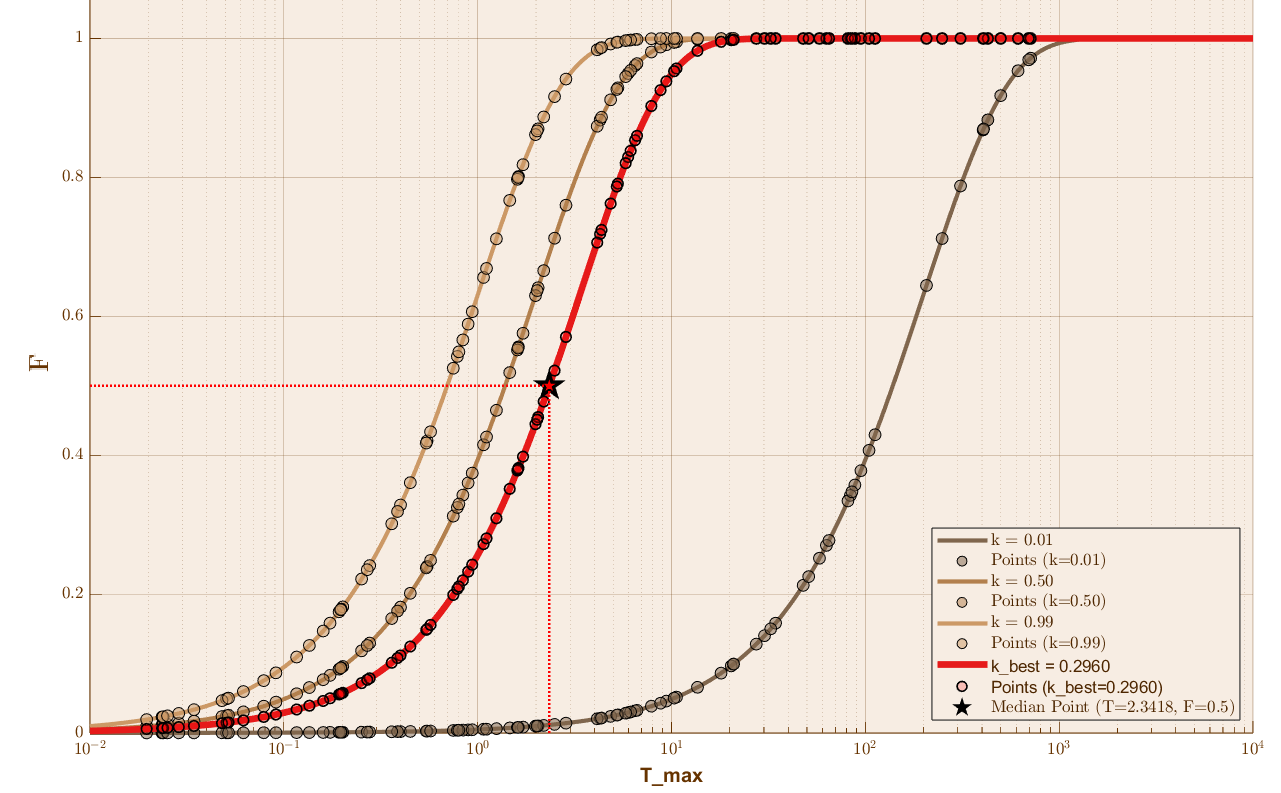
\includegraphics[width=0.85\linewidth]{fig/fitness.png}
    \caption{Best-k-Normalization of Randomly Generated $T_{max}$}
    \label{fig:fitness}
\end{figure}
\vspace{-0.3cm}
This formula maps the maximum total time to the interval [0,1] via the saturation of the exponential function, making it suitable as a fitness function in optimization models and balancing the impact of maximum time at different scales on the optimization objective.


\subsection{The Algorithm of Metaheuristic Optimization }

Given the allocation and traversal order, the total time is determined by the slowest firefighter (aiming to minimize this time).For NP-hard problem like this, brute force enumeration is costly, and \textbf{metaheuristic algorithms} can efficiently find approximate optimal solutions.

However, before that, we need to precisely express the allocation and permutation of a scheme. Hence, encoding:  

For $m$ firefighters $M_1$ to $M_m$, $n$ rooms $N_1$ to $N_n$, the encoding is $[N_1, N_2, N_3, \ldots, N_n \mid x_1, x_2, x_3, \ldots, x_m]$ (where $\sum x_i = n$). The first segment of the encoding $N_1, N_2, N_3, \ldots, N_n$ represents dividing these points (rooms) into $m$ groups, with the number of rooms in each group being $x_1, x_2, x_3, \ldots, x_m$ respectively. Note that the order of N only indicates the allocation of rooms, not the traversal order for each firefighter. For example, if a firefighter is assigned rooms $N_1$ and $N_2$, the order could be $N_1 \to N_2$ or $N_2 \to N_1$.  

Additionally, we do not mention entrances and exits in the encoding -we allow firefighters to enter from the exit closest to the first room and leave from the exit closest to the last room.  


\subsection*{Algorithm 1: Simulated Annealing Nested with Ant Colony Optimization}

To minimize time consumption, we recognize that equal allocation is a relatively optimal initial solution before traversal. Therefore, we adopt the following initial allocation: ensure that the number of rooms assigned to the firefighter with the fewest rooms is at most one less than the number assigned to the firefighter with the most rooms. That is:  

\(
x_{\text{max}} - x_{\text{min}} \leq 1, \quad \text{for } N \in \mathbb{Z}^+
\)

Now, consider using Ant Colony Optimization to determine how to order the firefighters' routes to minimize the total time consumption. 

Imagine that before setting out, firefighters release many ants to explore the optimal route. Ants leave pheromones on the paths they traverse. We assume that an equal amount of pheromone $Q$ is deposited on each path from one room to another. Thus, the increase in pheromone concentration $\Delta \tau$ on the path from point $n_i$ to $n_j$ due to an ant passing is:  

\(
\Delta \tau = \frac{Q}{L_k}
\)

Pheromones will evaporate so we set a parameter $\rho$ to represent the evaporation rate, which is a value in the interval [0,1]. Thus, the pheromone concentration on the path from $n_i$ to $n_j$ at time $t+1$ is:  

\[
\tau_{ij}(t+1) =  \rho \cdot \tau_{ij}(t) + \Delta \tau
\]

where $\tau_{ij}(t)$ is the pheromone concentration on the path at time $t$.  

Ants consider paths with higher pheromone concentrations to explore optimal solutions, as this indicates that more individuals have chosen this path. Thus:  

\[
p_{ij}^k  \propto \frac{(\tau_{ij}^\alpha)}{\sum_ (\tau_{iz}^\alpha)}
\]


where $P_{ij}$ is the probability that an ant at $n_i$ decides to go to $n_j$ next, and $\alpha$ is a parameter describing how much pheromone influences $P$. The denominator is the sum of pheromone concentrations over all possible paths.  

Simultaneously, ants also consider the distance between rooms. The greater the distance $D$ is, the less an ant will want to go there. Therefore, we define the inverse of distance as $\eta$. Similarly, $P_{ik}$ should be proportional to $\eta_{ij}^\beta$ divided by the sum of $\eta_i^\beta$, where $\beta$ describes the weight of the distance factor's influence on $P$. That is: \(P_{ij} \propto \eta_{ij}^\beta/\sum \eta_i^\beta\)

Thus, we have:  
\[
p_{ij}^k  =\frac{(\tau_{ij}^\alpha)(\eta_{ij}^\beta)}{\sum_ (\tau_{iz}^\alpha)(\eta_{iz}^\beta)}
\]

After multiple repetitions, the ants will converge on one path, which is the approximate optimal route. The firefighters can then follow this route. We calculate the time consumption for each firefighter and take the maximum as the total time consumption of this scheme.  

The problem now is how to update to a new allocation. We adopt the simulated annealing model. The general idea is: continuously attempt to find an allocation scheme that minimizes the total time consumption of the scheme; when the total time of a newly attempted scheme is less than the original total time, we always accept the new allocation; but if the new scheme's total time is greater, we accept it with a certain probability. This can be explained as follows---imagine the following graph, where the vertical axis represents the total time, and each point on the horizontal axis represents a new scheme. The goal is to find the minimum value of the entire function. Note that during the attempt, the entire function's shape is unknown; only the value of the next point is visible. When the next value is larger, to avoid being trapped in a local optimum and unable to cross the peak A to reach a smaller value B, we need to weigh whether to accept it.  

This trade-off is represented by the probability $P(\text{accept})$. When $P(\text{accept}) > 0.5$, we accept this risky change. According to previous research in thermodynamics, this probability is a natural exponential:  \(P(\text{accept}) = e^{-\frac{\Delta T}{T}}\), where $T$ is the total time of the original scheme, $T'$ is the total time of the newly attempted scheme, and $\Delta T$ is the change in total time---equal to $T' - T$.  

The model will continuously attempt until it oscillates around a value, which can be considered a relatively optimal solution.  

The only remaining problem is how to attempt. We should not spend too much effort on this as it should be random. Therefore, we define that each attempt can choose one of the following two operations: 1. Randomly exchange one room between two firefighters. 2. Transfer one room from one firefighter to another. The selection of firefighters and rooms is also random.  

\subsection*{Algorithm 2: Genetic Algorithm Fused with Particle Swarm Optimization}

If we consider the order of N in the encoding as the traversal order of the firefighters, this means that one segment of the encoding contains all the information of the scheme (i.e., allocation and order). We can directly use a calculation similar to Algorithm 1 to compute the total time consumption of an encoded scheme.  

The focus shifts to how to perform iterations: First, because it can be imagined that without the ant colony optimization for the optimal solution of each allocation, the iteration volume we obtain will be larger---to alleviate this computational and storage pressure, we fix the sample size of results for each iteration to $n$, and we only iterate on this group. Second, if the iteration of the group involves all encodings, it may lead to the loss or degradation of high-quality encodings. Therefore, before each iteration, we sort the encodings in the group from smallest to largest based on time consumption and retain the top 10\% of encodings to directly skip the iteration and enter the next group. It should be noted that this does not preserve stubborn encodings because even if retained into the next group, less excellent encodings will lose their top 10\% position in the next group's sorting and fall into iteration.  

After overcoming all difficulties, the only problem left is how to iterate. Imagine each encoding as a DNA double helix (one helix is the N sequence, the other is the x sequence). We mimic the crossover and mutation of DNA for iteration:  

Crossover between two DNAs involves selecting the same segment of encoding from the father's and mother's N sequences for exchange, while the x sequence remains unchanged, retaining the father's result as the offspring. Note that the N sequence can only crossover with the N sequence, and the x sequence can only crossover with the x sequence, exhibiting isolation. Crossover has directionality; the offspring will move in the direction of the mother based on the father.  

Mutation targets a single DNA, meaning extracting a segment from the N sequence and x sequence respectively, shuffling it, and then putting it back. Mutation is random because the probability of the shuffled encoding's score increasing or decreasing is equal.  

Then, who should be chosen as the mother? We refer to the particle swarm model---imagine each DNA is a particle. Many DNAs have already crossed with each other to form a large genetic tree. Each particle has a score at its current position, and the particle will move to try to find the point with the smallest score. The movement speed is: First, there is its own inertial velocity, which is random, manifested as DNA mutation. Second, it will move towards the point with the lowest score in its own historical path, manifested as the DNA crossing over with the one with the lowest score in its direct parental line. Third, not only one particle is moving and scouting; it will also move towards the point with the lowest score found by all particles' scouting, manifested as crossing over with the DNA with the lowest score in the entire lineage.  

In our model, we can understand it as follows: first, perform multiple random crosses on the initially generated initial group to obtain a genetic tree (note that pairwise crossing should not be done as this would cause the sample size to explode, resulting in more than $n$ encodings). Then, we randomly extract $a\%$ from the DNAs entering the iteration for mutation, $b\%$ for crossover with their best parent respectively, and $1-a\%-b\%$ for crossover with the historically best DNA.  






\subsection{Application in Single-story Office Building}
In the first scenario, we mainly focus on the single-story planar building. As shown in Fig \ref{fig:building_distance}(a), it is a floor of an office building with six offices, which has a layout measuring 17 meters in length by 11 meters in width.  We abstracted the doors of the six offices and the two exits into 8 nodes.

% 插入两张图，左右排布
\begin{figure}[htbp]  % h表示此处，t表示页顶，b表示页底，p表示独立一页，控制浮动体位置
	\centering  % 图表居中对齐
	\subfigure[Layout]{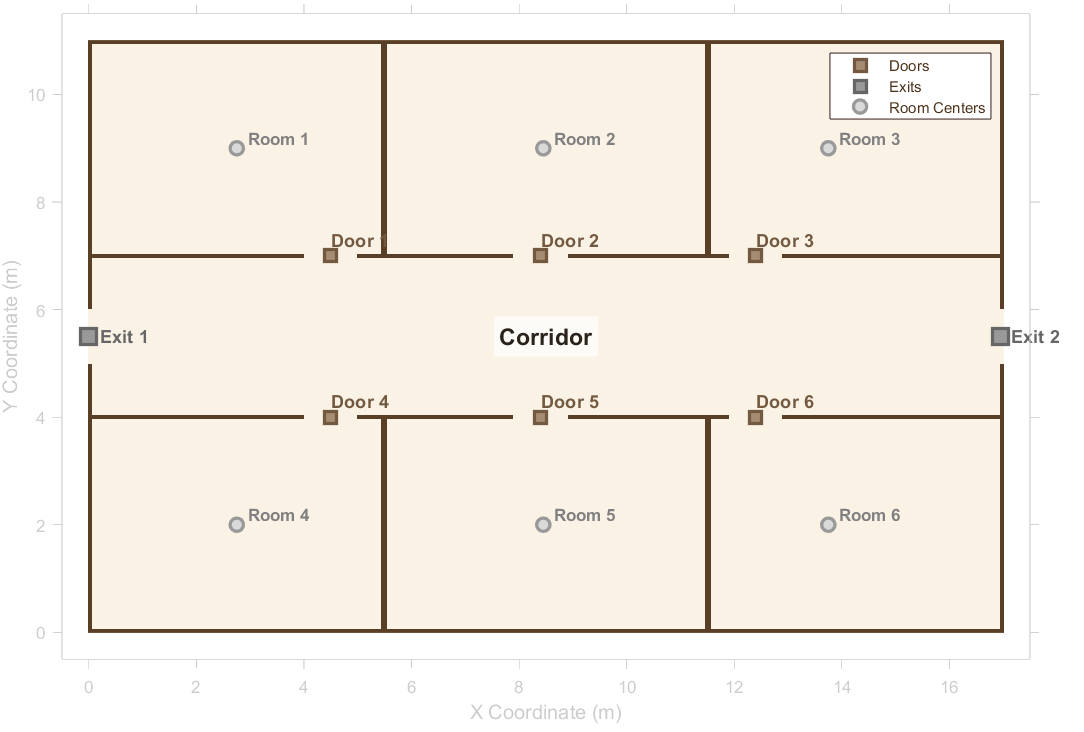
\includegraphics[width=.47\textwidth]{fig/layout1.png} % 注意图片名称或路径中不要有空格，否则会出错
	 }  % 补充右括号，修正子图标签格式
	\subfigure[Distance]{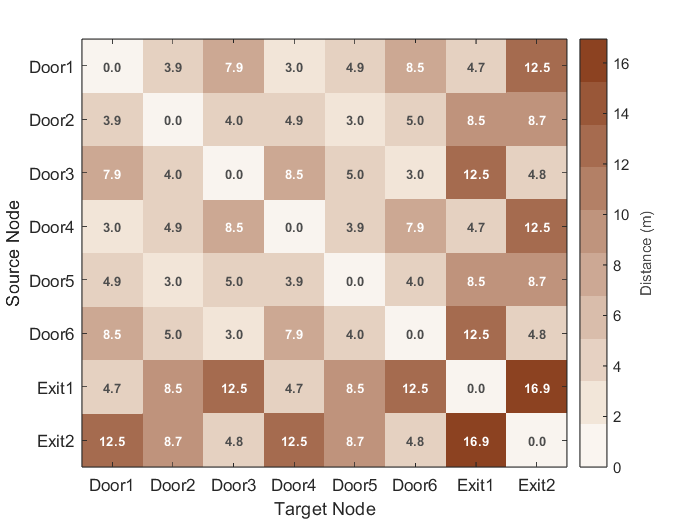
\includegraphics[width=.43\textwidth]{fig/Distance1.png} % 注意图片名称或路径中不要有空格
	 }  % 补充右括号，修正子图标签格式
	\caption{Building Layout and Inter-Room Distance Diagram}
	\label{fig:building_distance}  % 为整个图表添加主标签，便于后续引用
\end{figure}

\vspace{-0.5cm}%在\end{table}下加一行\vspace{-1cm} 其中-1的作用是缩短与下方文字距离的 切记！必须是负数

Then, the Euclidean distance is used to calculate the distance of each entrance (Fig \ref{fig:building_distance}(b)).  % 补充括号，规范图片引用格式
This value is substituted into the formula from the previous step of the model preparation process  % 修正"Mi surname"为"model"，应为笔误
and used to calculate $T_{\text{moving}}$. 

We have already determined the effective area of each office room $A=23\ \text{m}^2$. In simple offices, $L=1.0$, $C=1.0$, $E=1.0$ and $R=1.0$. So $Q=23\ \text{m}^2$.  % 单位前添加空格，补充括号使注释更清晰
With $\alpha_c \approx 0.4\ \text{m}^2/\text{s}$ 
(which matches a fire captain's speed), $T_{\text{check}} \approx 60\ \text{s}$.  

% 插入两张图，左右排布
\begin{figure}[htbp]  % h表示此处，t表示页顶，b表示页底，p表示独立一页，控制浮动体位置
	\centering  % 图表居中对齐
	\subfigure[ Simulated Annealing Algorithm]{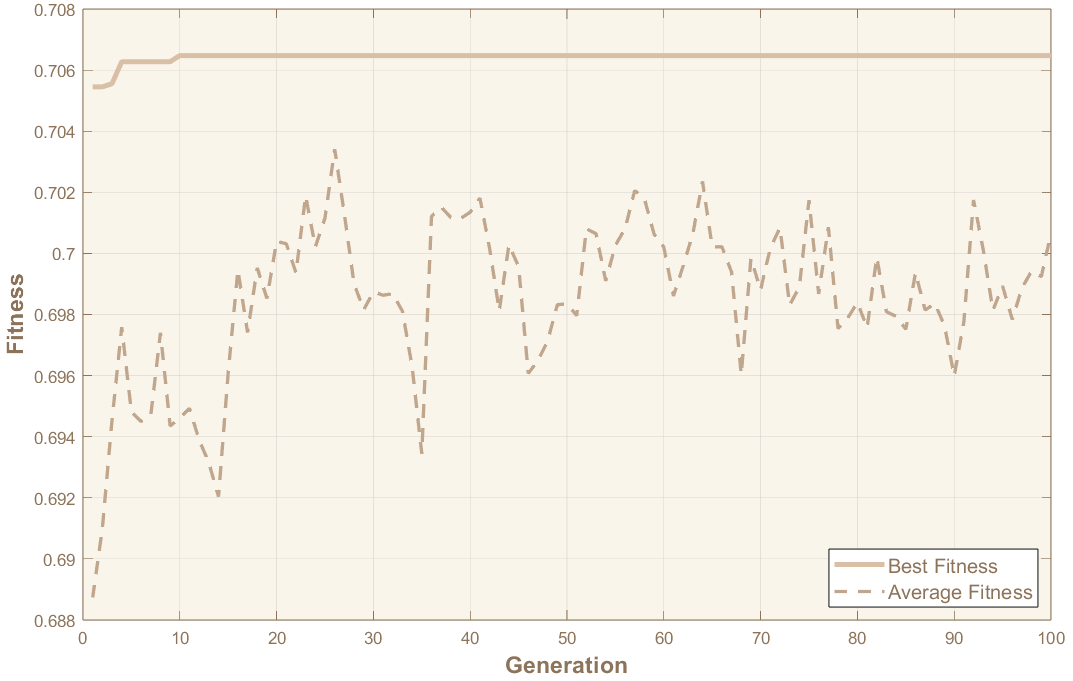
\includegraphics[width=.44\textwidth]{fig/Genetic Algorithm Fitness Evolution.png} % 注意图片名称或路径中不要有空格，否则会出错
	  \label{GA1}  % 补充右括号，修正子图标签格式
      }
	\subfigure[ Genetic Algorithm]{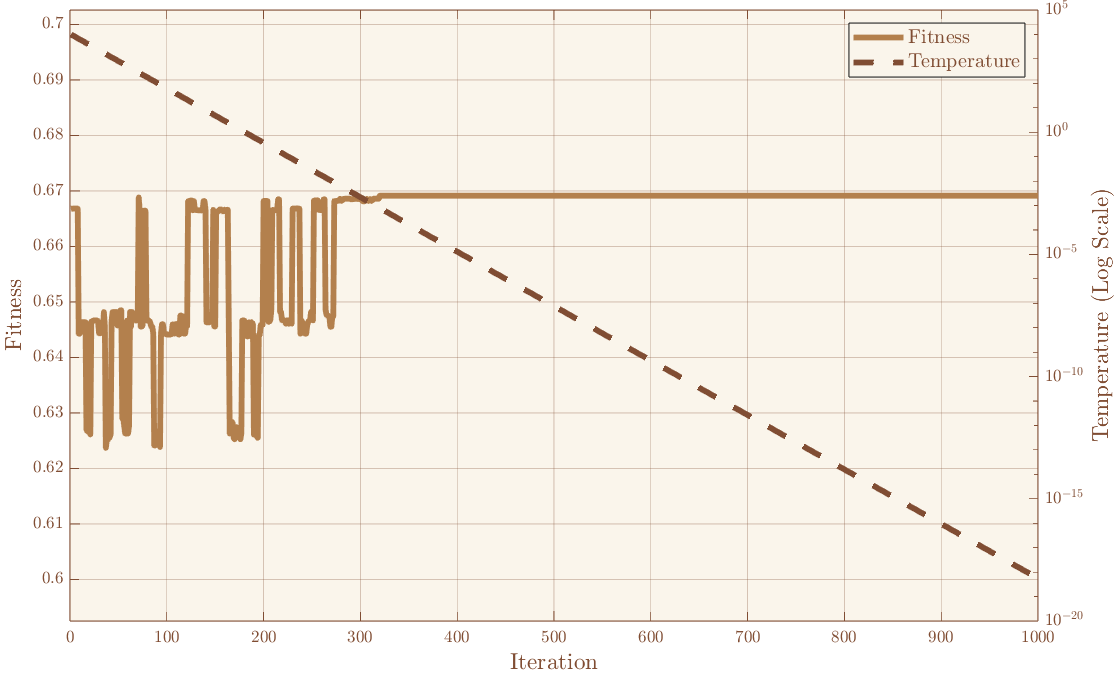
\includegraphics[width=.46\textwidth]{fig/SA1.png} % 注意图片名称或路径中不要有空格
	  \label{SA1}  % 补充右括号，修正子图标签格式
      }
	\caption{Curves of Algorithm Parameters vs. Iteration Number}
	\label{Algorithm Parameters}  % 为整个图表添加主标签，便于后续引用
\end{figure}
\vspace{-0.5cm}%在\end{table}下加一行\vspace{-1cm} 其中-1的作用是缩短与下方文字距离的 切记！必须是负数

Then, both GA and SA algorithm were applied for calculation. Figure \ref{Algorithm Parameters} shows the fitness evolution with iteration. In subfigure (a), the "Best Fitness" line rises steadily and stabilizes, while the "Average Fitness" line synchronously approaches it, verifying the algorithm’s ability to converge to the global optimal solution and avoid local optima. While in subfigure (b), the fitness curve gradually converges and the temperature curve decreases exponentially, reflecting the balance of the algorithm \textbf{between exploration and exploitation}.


The optimal fitness we obtained is 0.7063, corresponding to the paths: 

Firefighter 1 starts from Exit 1 → Door 4 → Door 5 → Door 6 → Exit 2; 

Firefighter 2 starts from Exit 2 → Door 3 → Door 2 → Door 1 → Exit 1 (as shown in Figrue \ref{path197.4s}(a)) % 去除多余空格，规范连接符使用

The time taken by each firefighter in this path was 197.4 seconds, and the optimal time was also \textbf{197.4 seconds.} 

% 插入两张图，左右排布
\begin{figure}[htbp]  % h表示此处，t表示页顶，b表示页底，p表示独立一页，控制浮动体位置
	\centering  % 图表居中对齐
	\subfigure[Best Scheme 197.4s]{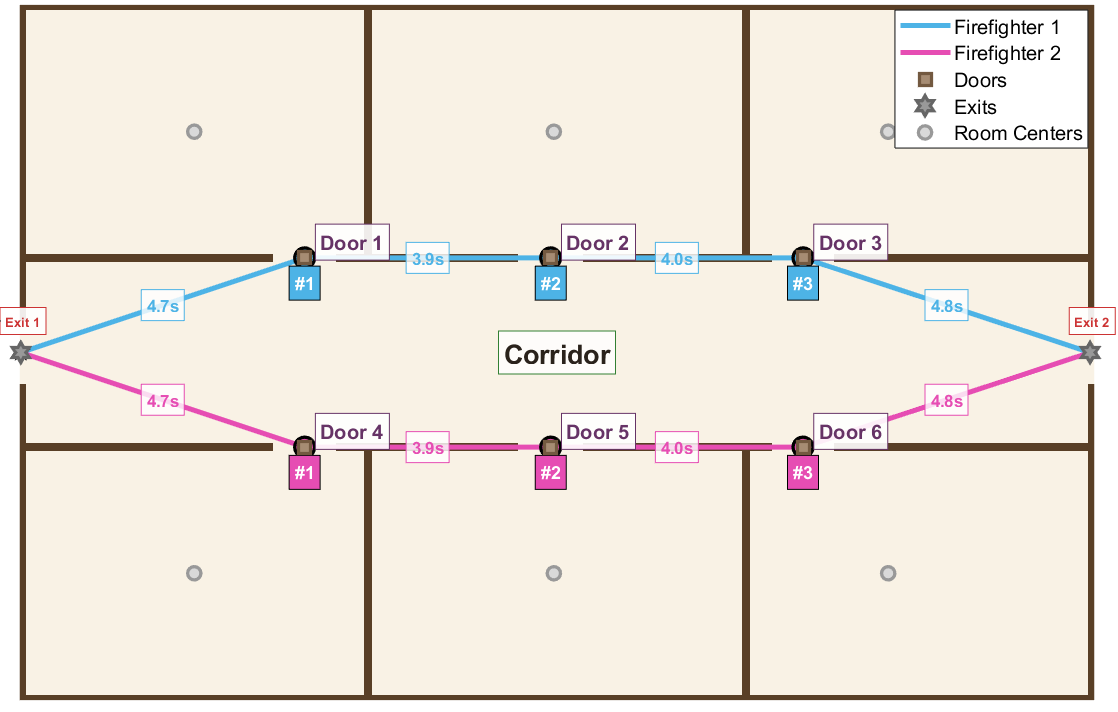
\includegraphics[width=.43\textwidth]{fig/bestpath197.4s.png} % 注意图片名称或路径中不要有空格，否则会出错
      }
	\subfigure[Second Best Scheme 198.6s]{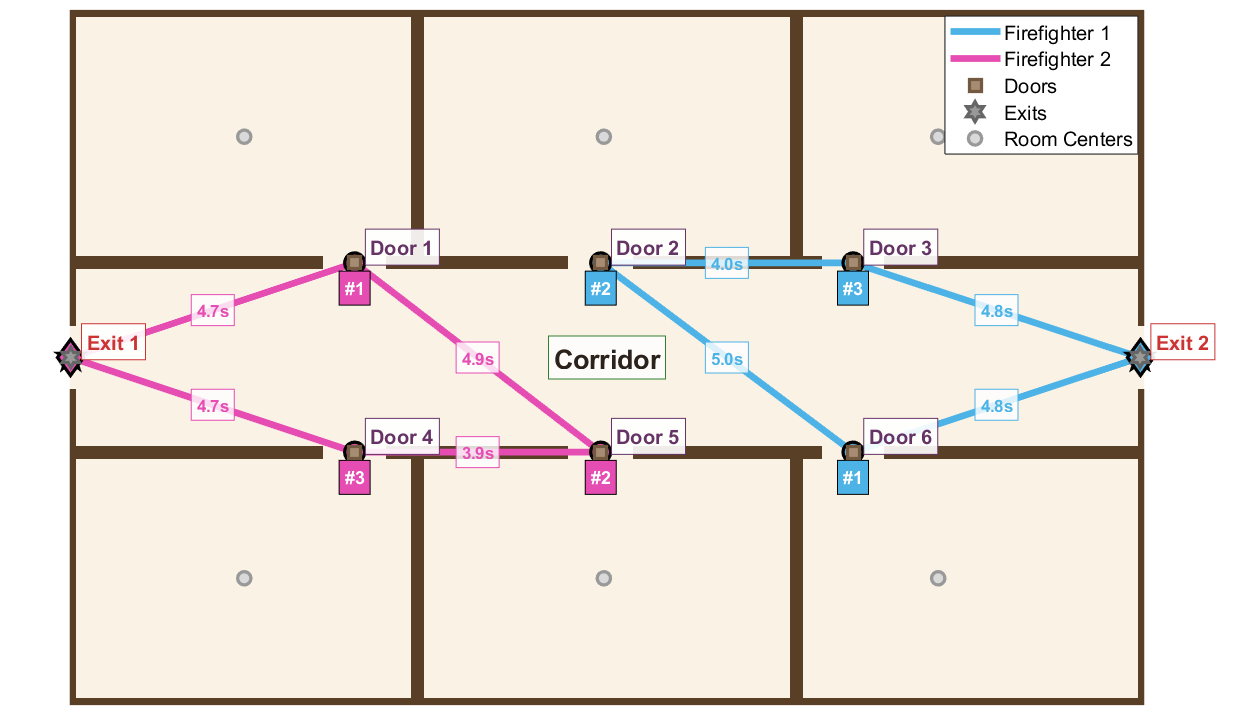
\includegraphics[width=.47\textwidth]{fig/path198.6s.png} % 注意图片名称或路径中不要有空格
      }
	\caption{Scheme for One-Story Office Building}
	\label{path197.4s}  % 为整个图表添加主标签，便于后续引用
\end{figure}
\vspace{-0.5cm}%在\end{table}下加一行\vspace{-1cm} 其中-1的作用是缩短与下方文字距离的 切记！必须是负数



For another scheme, as shown in Figure \ref{path197.4s}(b), the time consumed is almost the same, but it can ensure that the moving path of firefighters covers a smaller area, which is convenient for emergency responders to familiarize themselves with the site and carry out rescue when necessary.

When there is smoke in the fire scene, the value of the Incident Impact Coefficient (i.e., \( E \)) changes, and both the checking speed \( \alpha_c \) and moving speed \( \alpha_m \) of firefighters will decrease accordingly. We assume that the smoke concentration has an equal impact in all rooms and on the paths, and keep other parameters unchanged. Taking \( E = 2 \), \( \alpha_c \) is reduced to 10\% of its original value, and \( \alpha_m \) is reduced to three-quarters of its original value. This makes the \( T_{\text{check}} \) of each room 80s. After the algorithm runs, the optimized best path remains completely unchanged, but the maximum time consumed becomes 257.4s.
